\section{On Its Own Terms, the Loop Works}
\label{sec:gains}

\begin{figure}[t]
\centering
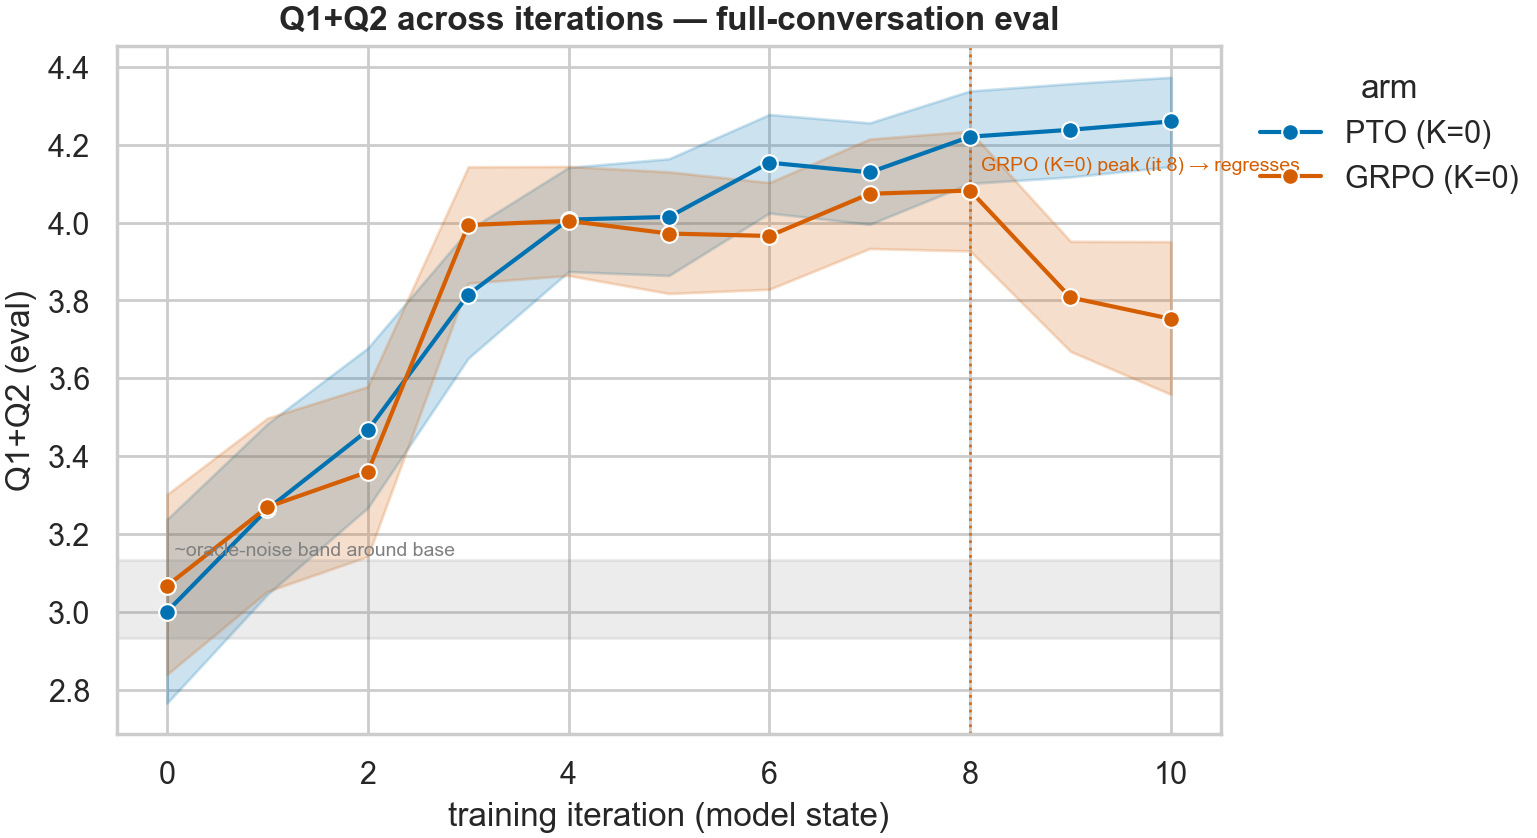
\includegraphics[width=0.9\columnwidth]{figures/trajectory_Q1Q2_gpt-4o-mini.png}
\caption{Training reward (\QQ{}) by iteration, mean over 96 personas, primary grader. Both
arms climb; PTO continues to iteration 10 while GRPO peaks at iteration 8 and regresses.
Shaded bands are bootstrap 95\% intervals.}
\label{fig:trajectory}
\end{figure}

\begin{table}[t]
\centering\small
\setlength{\tabcolsep}{3.5pt}
\begin{tabular}{@{}lrrrl@{}}
\toprule
& \textbf{base} & \textbf{iter 10} & \textbf{\dz{}} & \\
\midrule
\multicolumn{5}{@{}l}{\textbf{PTO} (preference tree $\rightarrow$ DPO)}\\
\QQ{}   & 3.00 & 4.26 & 1.43 & large \\
WAI-SR  & 2.85 & 3.50 & 0.97 & large \\
CSQ-8   & 2.38 & 2.95 & 0.81 & large \\
MI-SAT  & 2.84 & 3.65 & 0.90 & large \\
MITI    & 3.13 & 4.27 & 1.35 & large \\
PCT     & 0.49 & 0.63 & 0.62 & medium \\
MICI\,$\downarrow$ & 0.21 & 0.49 & 0.78 & \emph{worse} \\
\midrule
\multicolumn{5}{@{}l}{\textbf{GRPO} (group-relative); \QQ{} peaks 4.08 @ iter 8}\\
\QQ{}   & 3.07 & 3.75 & 0.72 & medium \\
WAI-SR  & 2.89 & 3.44 & 0.84 & large \\
CSQ-8   & 2.36 & 2.77 & 0.59 & medium \\
MI-SAT  & 2.86 & 3.48 & 0.66 & medium \\
MITI    & 3.22 & 3.92 & 0.82 & large \\
PCT     & 0.49 & 0.57 & 0.36 & small \\
MICI\,$\downarrow$ & 0.21 & 0.84 & 1.72 & \emph{worse} \\
\bottomrule
\end{tabular}

\vspace{2pt}
\begin{tabular}{@{}lrrrr@{}}
\toprule
\textbf{Paired} & \multicolumn{2}{c}{\textbf{final} 10\,v\,10} & \multicolumn{2}{c}{\textbf{best} 10\,v\,8}\\
\cmidrule(lr){2-3}\cmidrule(lr){4-5}
PTO${-}$GRPO & $\Delta$ & \dz{} & $\Delta$ & \dz{} \\
\midrule
\QQ{}              & $+0.51$ & 0.73    & $+0.18$ & 0.30 \\
MITI               & $+0.35$ & 0.46    & $+0.04$ & \emph{n.s.} \\
MICI\,$\downarrow$ & $-0.35$ & $-0.99$ & $-0.04$ & \emph{n.s.} \\
\bottomrule
\end{tabular}
\caption{\textbf{Top:} outcomes versus base, persona-paired over 96 personas, primary grader,
all Holm $p\approx0$; \dz{} banded $0.2/0.5/0.8$. \textbf{MICI is scored so lower is better},
so its large positive \dz{} is a deterioration --- the one row contradicting the rest.
\textbf{Bottom:} the head-to-head, both ways because final-only is unfair to GRPO. PTO leads on
the reward under either reading, but the effect halves at best-vs-best and \textbf{the MITI and
MICI gaps vanish} ($p=0.57$, $0.52$) --- see \S\ref{sec:gains}.}
\label{tab:main}
\end{table}


Both optimizers improve substantially on every instrument, and the improvements are
statistically unambiguous (Table~\ref{tab:main}; Holm-corrected $p\approx0$ throughout).

\paragraph{Magnitude.} Every global-evaluation rubric is a large effect for PTO, which moves
the reward \QQ{} from $3.00$ to $4.26$ ($\dz=1.43$). GRPO's endpoint is smaller ($\dz=0.72$),
understating its trajectory: it reaches $4.08$ at its iteration-8 peak before regressing
(Figure~\ref{fig:trajectory}). OLS slopes are $0.120$/iteration (PTO) against $0.072$ (GRPO).

\paragraph{Final versus best.} Comparing only final iterations is unfair to GRPO, which
regresses after iteration~8, so Table~\ref{tab:main} reports the head-to-head both ways. PTO
leads on the reward under either reading, but the effect halves at best-vs-best (\QQ{} $+0.51$,
$\dz=0.73$ $\rightarrow$ $+0.18$, $\dz=0.30$), and \textbf{the MITI and MICI gaps vanish}
($p=0.57$, $0.52$). Q1, MI-SAT, CSQ-8 and WAI-SR still survive Holm at best-vs-best. The
sycophancy separation is therefore a property of GRPO's \emph{post-peak run-off}, not of its
best state --- a materially weaker claim than the endpoint numbers alone suggest, and the one
we defend.

\paragraph{``Best'' is itself grader-dependent.} Selecting each arm's peak by the primary
oracle puts GRPO at iteration~8; the held-out judge (\S\ref{sec:heldout}) puts it at
iteration~3. Peak selection performed on the very signal being optimised is not a neutral
operation --- which is part of this paper's argument rather than an aside.

\paragraph{Absolute anchor.} Effect sizes say the model improved, not whether it became
competent. MITI 4.2.1 publishes ``fair'' and ``good'' thresholds, which place the endpoint on
an external scale (Table~\ref{tab:thresholds}): both arms move from below basic competence into
the fair-to-good band \emph{on the global ratings}, relational crossing ``good'' in both (PTO
$4.61$, GRPO $4.20$), while \textbf{neither reaches ``good'' on the technique ratios}.

GRPO's technique numbers need care. Its R:Q of $1.43$ formally clears ``fair'', but through the
denominator: reflections rise modestly (complex $0.093\rightarrow0.167$) while questions fall
($0.446\rightarrow0.319$), so the ratio improves largely because the therapist stopped asking.
As a competency claim that is a false positive, and the first sign of what \S\ref{sec:learned}
documents directly. We use these thresholds descriptively and lean no contrast on them
(see the caption, and the MITI caveat in \S\ref{sec:heldout}).

\begin{table}[t]
\centering\small
\setlength{\tabcolsep}{3pt}
\begin{tabular}{@{}llcccc@{}}
\toprule
& & \textbf{R:Q} & \textbf{\%CR} & \textbf{Tech.} & \textbf{Rel.} \\
\midrule
\multirow{2}{*}{PTO}  & base    & 0.61\,\xmark & 0.31\,\xmark & 2.92\,\xmark & 3.34\,\xmark \\
                      & iter 10 & 0.75\,\xmark & 0.36\,\xmark & 3.93\,fair   & \textbf{4.61\,good} \\
\midrule
\multirow{2}{*}{GRPO} & base    & 0.70\,\xmark & 0.30\,\xmark & 3.05\,fair   & 3.40\,\xmark \\
                      & iter 10 & 1.43\,fair$^{*}$ & 0.41\,fair & 3.64\,fair & \textbf{4.20\,good} \\
\bottomrule
\end{tabular}
\caption{Endpoint placed against MITI 4.2.1 competency thresholds. \xmark{} = below ``fair''.
Both arms cross into ``good'' on the \emph{relational} global; neither reaches ``good'' on the
\emph{technique} ratios. $^{*}$GRPO's reflection-to-question ratio clears ``fair'' primarily
by shrinking its denominator (\S\ref{sec:learned}), which is why we treat it as a false
positive rather than a competency gain. Thresholds are the manual's expert consensus for
20-minute human sessions --- an anchor, not a certification --- and rest on MITI, whose
cross-judge dependability is the weakest of the eight instruments.}
\label{tab:thresholds}
\end{table}

